%%%%%%%%%%%%%%%%%%%%%%%%%%%%%%%%%%%%%%%%%%%%%%%%%%%%%%%%%%
%                                                                                      %
%         Bristol Project LaTex Template            %
%                                                                                      %
%%%%%%%%%%%%%%%%%%%%%%%%%%%%%%%%%%%%%%%%%%%%%%%%%%%%%%%%%%
%
%   Author: Alex Charles           Email: aep.charles@gmail.com
%
% -----------------------------------------------------------------------------------
%      PACKAGES & OTHER DOCUMENT CONFIGURATIONS
% -----------------------------------------------------------------------------------
\documentclass[fontsize=9.5pt]{extarticle}

\usepackage[utf8]{inputenc}
\usepackage[T1]{fontenc}
\usepackage[british]{babel}
% ----------NEW BIBLATEX BIBLIOGRAPHY-----------------------------------------------
\usepackage[backend=bibtex,style = ieee]{biblatex} % Upgrades Bibliography

\addbibresource{BibFile.bib} %%% For biblatex
%e.g to add page number \footfullcite[chapter, p.~215]{AAIB}
% This allows can use footfullcite commands
% Note urldate field must be in yyyy-mm-dd to work - use online type
% Remeber to use \printbibliography in the footer
% -----------------------------------------------------------------------------------
% \usepackage{sectsty}
\usepackage{amssymb,amsmath}
\usepackage{ifxetex,ifluatex}  %<<<<<<<<< Edit FONT HERE
% \usepackage{fontspec}
% \setmainfont{Times New Roman}
\ifnum 0\ifxetex 1\fi\ifluatex 1\fi=0 % if pdftex
  \usepackage[T1]{fontenc}
  \usepackage[utf8]{inputenc}
\else % if luatex or xelatex
  \ifxetex
    \usepackage{mathspec}
    \setmainfont[
 BoldFont={Avenir-Medium},ItalicFont={Avenir-BookOblique},
 BoldItalicFont={Avenir-MediumOblique}]{Avenir-Book}
  \else
  % Font Package for XeLatex
    \usepackage{fontspec}
    \setmainfont{Avenir-Light}
  \fi
  \defaultfontfeatures{Ligatures=TeX,Scale=MatchLowercase}
\fi
\usepackage[fit]{truncate} %Truncates headers that are too long
\usepackage{fancyhdr}
\usepackage{lastpage}
\usepackage{extramarks}
\usepackage{gensymb}
\usepackage{lipsum}
\usepackage{float}
\usepackage{graphicx}
\graphicspath{{TempImg/}{Img/}}%<<<<<<<<< Location of Template Images and Other Images, Add folders here
\usepackage{subfig}
\usepackage{wrapfig}
\usepackage[font ={small,it}]{caption}
\usepackage{amsfonts,amsthm} % Math packages
% \usepackage{cite}
% \usepackage[maxlevel=3]{csquotes}
%    \MakeAutoQuote{‘}{’}
%    \MakeAutoQuote*{“}{”} %corrects quote marks
\usepackage{enumitem} % resume numbered lists
\usepackage{multicol} %for mulitple colums in lists
\usepackage{geometry}
\usepackage{booktabs} %<<<<<<<<< Table drawing package
\usepackage[table,xcdraw]{xcolor} %<<<<<<<<< Table drawing package
\usepackage{svg}
\usepackage{scrextend} %call footnotes
\usepackage[colorlinks, linkcolor = black, citecolor = black, filecolor = black, urlcolor = blue]{hyperref} % Creates Hyperlinks for references - add [colorlinks] for coloured hyperlinks
\usepackage{changepage} %Allows Adjust width to be used for the document (indenting paragraphs)
\usepackage{pdfpages} %Allows Pdfpages to be added to the document use \includepdf[pages={1}]{myfile.pdf}
\usepackage{pdflscape} %Change Pages from Portrait to Landscape

% \usepackage[compact]{titlesec}
\usepackage{titlesec}
\titlespacing\section{0pt}{8pt plus 4pt minus 2pt}{0pt plus 2pt minus 2pt}
\titlespacing\subsection{0pt}{0pt plus 3pt minus 2pt}{-3pt plus 2pt minus 2pt}
\titlespacing\subsubsection{0pt}{0pt plus 2pt minus 2pt}{-6pt plus 2pt minus 2pt}
\titlespacing\subsubsubsection{0pt}{-6pt plus 2pt minus 2pt}{-6pt plus 2pt minus 2pt}
\setlength{\multicolsep}{-1pt plus 2.0pt minus 1.5pt}% 50% of original values

% \titlespacing*{\section}{0pt}{1.1\baselineskip}{\baselineskip}

\renewcommand*{\thefootnote}{\alph{footnote}} %%% Changes footnotes to letters
\usepackage[bottom]{footmisc} %%% Pushes footnote to bottom and to the margin

\DeclareCiteCommand{\footcite}[\mkbibfootnote]
{\usebibmacro{cite:init}%
\usebibmacro{prenote}}
{\usebibmacro{citeindex}%
\printtext[brackets]{\usebibmacro{cite:comp}}}
{\multicitedelim}
{\usebibmacro{cite:dump}%
\usebibmacro{postnote}}

\newenvironment{indentpara}{\begin{adjustwidth}{2cm}{}}{\end{adjustwidth}} %Declare adjust width wiht indentpara
\renewcommand{\labelitemii}{$\circ$}
\renewcommand{\labelitemiii}{$\diamond$}
\renewcommand{\labelitemiii}{$\cdot$}

% -----------------------------------------------------------------------------------
%                 Code
% -----------------------------------------------------------------------------------
\usepackage{listings}
\lstset{inputpath=Code/}
\usepackage{color}
\definecolor{mygreen}{RGB}{28,172,0} % color values Red, Green, Blue
\definecolor{mylilas}{RGB}{170,55,241}

\lstset{language=Matlab,%
    %basicstyle=\color{red},
    breaklines=true,%
    basicstyle=\small,
    morekeywords={matlab2tikz},
    keywordstyle=\color{blue},%
    morekeywords=[2]{1}, keywordstyle=[2]{\color{black}},
    identifierstyle=\color{black},%
    stringstyle=\color{mylilas},
    commentstyle=\color{mygreen},%
    showstringspaces=false,%without this there will be a symbol in the places where there is a space
    numbers=left,%
    numberstyle={\tiny \color{black}},% size of the numbers
    numbersep=9pt, % this defines how far the numbers are from the text
    emph=[1]{for,end,break},emphstyle=[1]\color{red}, %some words to emphasise
    %emph=[2]{word1,word2}, emphstyle=[2]{style},
}

%% To Add Code Use :
% \lstinputlisting{myfun.m}
%% To input a file or :
% \begin{figure}[h]
% \begin{lstlisting}[language=Matlab]
% \end{lstlisting}
% \catpion{code}
% \end{figure}


% -----------------------------------------------------------------------------------
%                 Quotes
% -----------------------------------------------------------------------------------

\usepackage{epigraph}
% \epigraphsize{\small}% Default
\setlength\epigraphwidth{12cm}
\setlength\epigraphrule{0pt}

\usepackage{etoolbox}
\apptocmd{\sloppy}{\hbadness 10000\relax}{}{}%%%% > Removes Url bibliography warnings
\makeatletter
\patchcmd{\epigraph}{\@epitext{#1}}{\itshape\@epitext{#1}}{}{}
\makeatother

%%%% > For Quotes Use \epigraph{"Quote"}{ - \textup{Author}, Book}

% -----------------------------------------------------------------------------------
%                   NAMES & CLASS DEFINITION %<<<<<<<<< INSERT DETAILS HERE
% -----------------------------------------------------------------------------------
\newcommand{\AssignmentTitle}{Investigation of the Use Energy Storage Technologies to Reduce Peak Demand Charges for the University of Bristol}
\newcommand{\ModuleTitle}{Design Project 4 - Final Report}
\newcommand{\University}{University of Bristol}
\newcommand{\Faculty}{Faculty of Engineering}
\newcommand{\UniCrest}{crestbris.png}
\newcommand{\UniLogo}{logobris.png}%<<<<<<<<< Make Sure Files are in the Template
%\newcommand{\GroupName}{Group 2}
\newcommand{\StudentNameA}{Alexander Charles}
\newcommand{\StudentNumberA}{67634}
\newcommand{\SupervisorNameA}{Dr Theo Tryfonas}
\newcommand{\SupervisorEmailA}{Theo.Tryfonas@bristol.ac.uk}
% \newcommand{\SupervisorNameB}{Name}
% \newcommand{\SupervisorEmailB}{email@gmail.com}

% -----------------------------------------------------------------------------------
%        PACKAGES FOR MARKDOWN CONVERSION - FOR USE If Using Markdown to Latex
% -----------------------------------------------------------------------------------
\usepackage{fixltx2e} % provides \textsubscript
% use upquote if available, for straight quotes in verbatim environments
\IfFileExists{upquote.sty}{\usepackage{upquote}}{}
% use microtype if available
\IfFileExists{microtype.sty}{%
\usepackage{microtype}
\UseMicrotypeSet[protrusion]{basicmath} % disable protrusion for tt fonts
}{}
\hypersetup{unicode=true,
            pdftitle={\AssignmentTitle},
            pdfauthor={\StudentNameA},
            pdfborder={0 0 0},
            breaklinks=true}
\urlstyle{same}  % don't use monospace font for urls
\usepackage{fancyvrb}
\VerbatimFootnotes % allows verbatim text in footnotes
\usepackage{longtable,booktabs}
\IfFileExists{parskip.sty}{%
\usepackage{parskip}
}{% else
\setlength{\parindent}{0pt}s
\setlength{\parskip}{6pt plus 2pt minus 1pt}
}
\setlength{\emergencystretch}{3em}  % prevent overfull lines
\providecommand{\tightlist}{%
  \setlength{\itemsep}{0pt}\setlength{\parskip}{0pt}}
% \setcounter{secnumdepth}{0}
% Redefines (sub)paragraphs to behave more like sections
\ifx\paragraph\undefined\else
\let\oldparagraph\paragraph
\renewcommand{\paragraph}[1]{\oldparagraph{#1}\mbox{}}
\fi
\ifx\subparagraph\undefined\else
\let\oldsubparagraph\subparagraph
\renewcommand{\subparagraph}[1]{\oldsubparagraph{#1}\mbox{}}
\fi

% -----------------------------------------------------------------------------------
%                   WORD COUTNER - for XeLaTex
% -----------------------------------------------------------------------------------
\usepackage{xesearch}
\newcounter{words}
\newenvironment{counted}{%
  \setcounter{words}{0}
  \SearchList!{wordcount}{\stepcounter{words}}
    {a?,b?,c?,d?,e?,f?,g?,h?,i?,j?,k?,l?,m?,
    n?,o?,p?,q?,r?,s?,t?,u?,v?,w?,x?,y?,z?}
  \UndoBoundary{'}
  \SearchOrder{p;}}{%
  \StopSearching}

% -----------------------------------------------------------------------------------
%                   MARGINS, HEADERS & FOOTERS
% -----------------------------------------------------------------------------------
 \geometry{
 left=25.4mm,
 right=25.4mm,
 top=25.4mm,
 bottom=25.4mm,
 }
\linespread{1.5}

\pagestyle{fancy}
\lhead{\includegraphics[width = 0.2\textwidth]{\UniLogo}}
% \chead{\AssignmentTitle}
% \rhead{}
\lfoot{\StudentNameA}
\cfoot{\thepage}
% \rfoot{Page \thepage} %%%% note the footer is swapped when page numbering style changes
\renewcommand\headrulewidth{0.4pt}
\renewcommand\footrulewidth{0.4pt}

\setlength\parindent{0pt}

\newcommand{\horrule}[1]{\rule{\linewidth}{#1}}

% -----------------------------------------------------------------------------------
%               DOCUMENT STRUCTURE COMMANDS
% -----------------------------------------------------------------------------------
% To sort out the formatting of header and footer when a page...
% ... split occurs "within" a problem environment.
\newcommand{\enterProblemHeader}[1]{
\nobreak\extramarks{#1 (Cont.)}\nobreak
\nobreak\extramarks{#1}{}\nobreak
}
% To sort out the formatting of header and footer when a page...
% ... split occur "between" problem environments.
\newcommand{\exitProblemHeader}[1]{
\nobreak\extramarks{#1 (Cont.)}\nobreak
\nobreak\extramarks{#1}{}\nobreak
}

% -----------------------------------------------------------------------------------
\begin{document}

  \setlength{\abovedisplayskip}{-18pt}
  \setlength{\belowdisplayskip}{0pt}
  \setlength{\abovedisplayshortskip}{-18pt}
  \setlength{\belowdisplayshortskip}{0pt}

  \setlist[enumerate]{itemsep=-2mm}
  \setlist[itemize]{itemsep=-2mm}


%----------------------------------------------------------------------------------------
                                  %	TITLE PAGE FORMAT
%----------------------------------------------------------------------------------------
\pagenumbering{roman}
\begin{titlepage}

	\center % Center everything on the page
%----------------------------------------------------------------------------------------
%	HEADING SECTION
%----------------------------------------------------------------------------------------
		\usefont{OT1}{bch}{b}{n}
		\normalfont \normalsize \textsc{\University} \\ [10pt]
		\normalfont \normalsize \textsc{\Faculty} \\ [25pt]
%----------------------------------------------------------------------------------------
%	LOGO SECTION - Adds Univeristy Crest to the Report
%----------------------------------------------------------------------------------------
\newcolumntype{C}{>{\centering\arraybackslash} m{6cm} }  %# New column type
\begin{tabular}{CC}
  \includegraphics[width = 0.2\textwidth]{\UniCrest} &   
\includegraphics[width=0.3\textwidth]{Arup_logo.png}
\end{tabular}\\[0.5cm]
%----------------------------------------------------------------------------------------
%	HEADING SECTION
%----------------------------------------------------------------------------------------
		\normalfont \normalsize \textsc{\ModuleTitle} \\ [25pt]
%----------------------------------------------------------------------------------------
%	TITLE SECTION
%----------------------------------------------------------------------------------------
		\horrule{0.5pt} \\[0.4cm]
		\huge \textbf{\AssignmentTitle} \\
		\horrule{2pt} \\[0.5cm]
%----------------------------------------------------------------------------------------
%	HEADING SECTION
%----------------------------------------------------------------------------------------
%		\normalfont \normalsize \textsc{\GroupName} \\ [25pt]
%----------------------------------------------------------------------------------------
%	AUTHOR SECTION
%----------------------------------------------------------------------------------------
\begin{minipage}{0.4\textwidth}
\begin{flushleft} \large
\emph{Supervisors:}\\
% Change Name
\textbf{\SupervisorNameA}\\
% \textbf{\SupervisorNameB}
\end{flushleft}
\end{minipage}
~
\begin{minipage}{0.4\textwidth}
\begin{flushright} \large
\emph{Email:} \\
\SupervisorEmailA\\
% \SupervisorEmailB

\end{flushright}
\end{minipage}\\[1cm]

\begin{minipage}{0.4\textwidth}
\begin{flushleft} \large
\emph{Author:}\\
	\textbf{\StudentNameA}
\end{flushleft}
\end{minipage}
~
\begin{minipage}{0.4\textwidth}
\begin{flushright} \large
\emph{Candidate Number:} \\
(\StudentNumberA)\\
\end{flushright}
\end{minipage}\\[2cm]

%----------------------------------------------------------------------------------------
%	DATE SECTION
%----------------------------------------------------------------------------------------
\textit{{\large \today}}\\[1cm] % Date, change the \today to a set date if you want to be precise
%----------------------------------------------------------------------------------------
\vfill % Fill the rest of the page with whitespace
\end{titlepage}

% \setcounter{page}{3}

\newpage

% -----------------------------------------------------------------------------------
%                             	 Acknowledgements
% -----------------------------------------------------------------------------------

\addcontentsline{toc}{section}{Acknowledgements}
\section*{Acknowledgements}\label{acknowledgements}
A paragraph should be written in place of this text, acknowledging all persons who have helped or contributed towards your project. All formally allocated supervisors should be acknowledged first followed by other university staff, representatives of external companies and people not falling in those categories such as peers and PhD students. The acknowledgement should indicate the nature of the assistance received, for example “I acknowledge Paul Rowe of OnAxis Ltd for providing the linear motors used in section 4 and Dr Simon Richards for help in writing the source code for the controller.”

\addcontentsline{toc}{section}{Declaration}
\section*{Declaration}\label{declartion}
\begin{quote}
\textit{The accompanying research project report entitled:  “\AssignmentTitle” is submitted in the fourth year of study towards an application for the degree of Bachelor of Engineering in Engineering Design at the University of Bristol. The report is based upon independent work by the candidate. All contributions from others have been acknowledged above. The views expressed within the report are those of the author and not of the University of Bristol.}
\end{quote}
I hereby declare that the above statements are true.
\\
\\Signed (author)
\\
\\ ………………………………………………………………………
\\
\\ Full Name
\\
\\ {\large \StudentNameA}
\\
\\ Date
\\
\\ {\large \today}

\newpage

% -----------------------------------------------------------------------------------
%                             	 ABSTRACT
% -----------------------------------------------------------------------------------

\addcontentsline{toc}{section}{Executive Summary}
\section*{Executive Summary}\label{ExecSummary}

\newpage
% -----------------------------------------------------------------------------------
%                              TABLE OF CONTENTS
% -----------------------------------------------------------------------------------

\tableofcontents


\newpage
\addcontentsline{toc}{section}{List of Figures}
\listoffigures
\addcontentsline{toc}{section}{List of Tables}
\listoftables
\addcontentsline{toc}{section}{List of Acronyms}
\section*{List of Acronyms}\label{acronyms}
\begin{tabular}{p{1cm}p{12cm}}
\textbf{ESS}:& Energy Storage System \\
\textbf{DUoS}:& Energy Storage SystemDistribution Use of System\\
\textbf{TNUoS}:& Transmission Network Use of System\\
\textbf{SQP}:& Sequential Quadratic Programming\\
\textbf{ROI}:& Return On Investment\\
\textbf{VRB}&: Vanadium Redox Batteries\\
\textbf{PHS}:& Pumped Hydroelectric Storage\\
\textbf{CAES}:& Compressed Air Energy Storage\\
\textbf{CES}:& Cryogenic Energy Storage\\
\textbf{TES}:& Thermal Energy Storage\\
\textbf{SMES}:& Superconducting Magnetic Energy Storages\\
\end{tabular}

\newpage

%% -----------------------------------------------------------------------------------
%%                          	  INTRODUCTION
%% -----------------------------------------------------------------------------------
\clearpage
\cfoot{\thepage}
% \rfoot{Page \thepage\ of \pageref{LastPage}}
\pagenumbering{arabic}
\begin{counted} %<<<<<<<<<<<<<<STARTS WORD COUNTER
\section{Aims and Objectives}\label{aims-and-objectives}

The announcement of the new £300million University of Bristol Campus in
Temple Quarter \cite{November58:online}, presents an exciting new
opportunity for digital innovations in sustainable energy. The
government's 2020 smart meter rollout, is the first step for creating a
smart energy grid, key to achieving a low-carbon, sustainable and
efficient energy for the UK \cite{SmartEne79:online}. The UK's vision
corresponds to the University of Bristol's new strategy, seeking to
boost its world-class research capacity and promote innovation in policy
to increase sustainability \cite{universi93:online}. The creation of a
world-leading sustainable digital campus is an attractive means for the
University to achieve its vision. Consequently, the aim of this group
project is to bring a explore of new digital technologies reducing both
energy costs and energy usage, uniting these themes to set a new
frontier in campus's sustainability.

\begin{figure}[H]
\centering
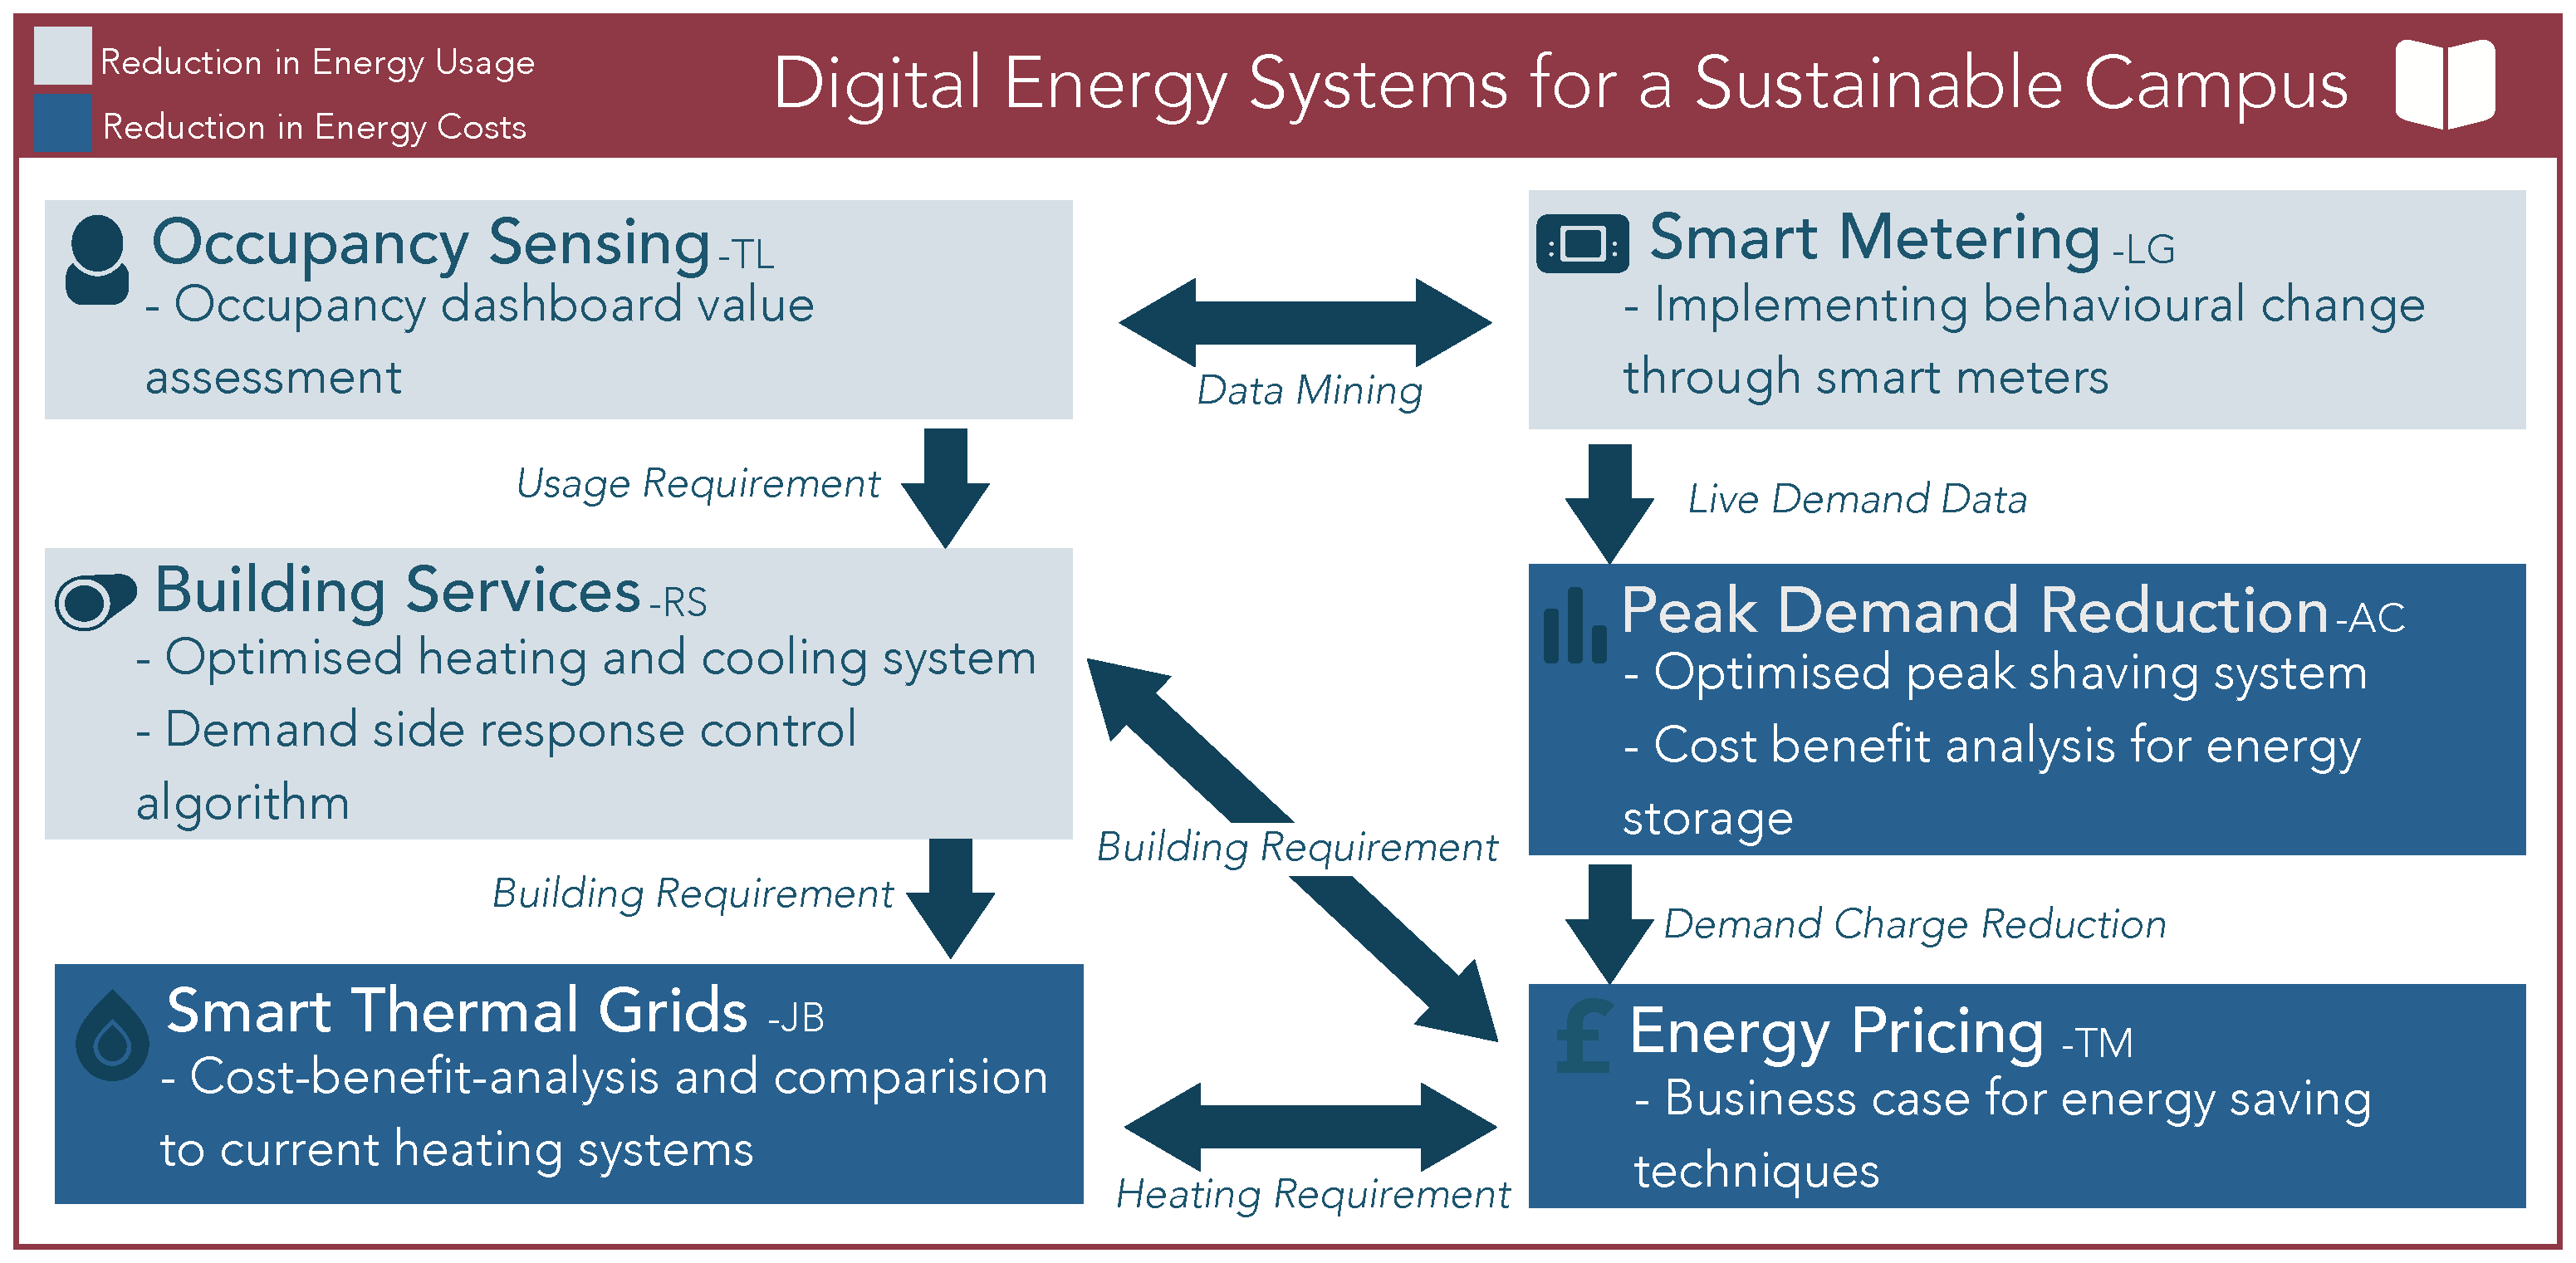
\includegraphics[width=1\textwidth]{diagramGroup.eps}
\caption{Group Design Project Diagram Showing Relationships Between Individual Projects}
\vspace{-20pt}
\label{groupDia}
\end{figure}

Figure \ref{groupDia} shows how the separate subjects of the project are
split, where research in Occupancy Sensing, Smart Metering and Building
Services will evaluate how energy usage in the new campus can be
optimised. Smart Thermal Grid, Energy Pricing and Peak Demand Reduction,
all analyse methods of reducing the University's energy costs. Where new
energy pricing structures coupled with peak demand reduction
technologies, can reduce the load on the grid, helping support
sustainable energies. The 5\textsuperscript{th} year group project will
unite these themes, creating a smart ``brain'' through combining usage
data with new technologies and strategies, providing a business case to
develop sustainable energy services on the new campus, pushing the
University to meet it's carbon neutral 2030 goal
\cite{universi93:online}.

\subsection{Individual Project Aim}\label{individual-project-aim}

The aim of this individual project is to investigate the feasibility of
using an energy storage system (ESS) to reduce charges related to peak
energy demand for the University of Bristol, implemented in the new
Temple Quarter campus. Within the project, the University's peak demand
charges will be analysed and simulated, modelling the bespoke energy
requirements of the campus. Different peak-shaving system architectures
will then be modelled against this usage and charge data, finding an
optimum solution for the system's design concerning the system's capital
cost against savings made from energy bills. This model will provide a
comparison between using a decentralised system, for room by room use,
or a centralised system, being applied to the whole building. The
outputs of the project for 5\textsuperscript{th} year will be a flexible
model which produces an optimum peak-shaving system architecture for a
given University scenario, providing a cost benefit analysis of using
energy storage.

\subsection{Objectives}\label{objectives}

\textbf{Literature Review}

\begin{enumerate}
\item Perform a detailed literature review, and market analysis of energy storage systems used to reduce peak energy demands, highlighting relevant modelling techniques and limitations.
\item Investigate different energy storage solutions, looking at their applicability to a University peak-shaving system, comparing parameters such as; power-ratings, discharge times, charge times and costs.
\end{enumerate}

\textbf{Definition of System Architectures}

\begin{enumerate}[resume]
\item Define peak-shaving system architectures, establishing the key performance variables. This objective will include an investigation of peak demand sensing, smart metering usage, energy storage health monitoring, energy conversion, methods to split supply between an energy storage system and the mains and a comparison between decentralised and centralised energy storage models.

\end{enumerate}

\textbf{Modelling and Analysis}

\begin{enumerate}[resume]
\item Analyse the University’s current peak demand charges; understanding the University’s current demand charge structure and collecting typical energy usage data. Parameters such as time of day and sources of energy peaks will be incorporated.
\item Produce a simulation to optimise the peak-shaving system, comparing metrics including; unit cost and reduction in peak kWh charges based on University billing structure. This model will provide a comparative analysis of the different system architectures. The model will detail savings against the University’s current peak demand charges, being comprised of three stages:
\begin{enumerate}
\item A simulation of the University's a normal energy use case and peak demand charges, for use as a datum.
\item Inclusion of energy storage systems, simulating logic and detailing any prediction methods.
\item An assessment of the use of peak load shedding, supply levelling and forecasting to improve the performance of the model.
\end{enumerate}
\end{enumerate}

\textbf{Evaluation}

\begin{enumerate}[resume]
\item Evaluate results of the simulation, concluding on the effectiveness of different peak-shaving system architectures against particular scenarios. A cost-based analysis will be used to measure the feasibility of the different energy storage systems for the University.
\end{enumerate}

\newpage

\section{Background and Summary of Key Work and
References}\label{background-and-summary-of-key-work-and-references}

The following literature review provides a comprehensive overview of
current research towards using Energy Storage Systems (ESS) to reduce
peaks in energy demand and lower utility costs for the consumer. Peak
demand reduction is synonymous with peak shaving; the ability to control
energy usage from a supplier during intervals of high demand, to limit
or reduce demand charges \cite{schneiderRECPS}, \cite{baldorPS}. As this
project is investigating reducing the peak demand charge for the
University of Bristol, section \ref{peak-demand-charges}, provides an
overview of the Univerity's energy bill, detailing which charges are
effected by peak demand. Section
\ref{current-peak-demand-management-methods-and-energy-storage-systems-usage}
evaluates traditional methods of peak shaving, covering a brief look at
ESSs current usage. Section \ref{peak-shaving-systems-literature-review}
includes a broad range of research of ESSs in different case studies,
optimising the system architecture and analysis on ESSs financial return
on investment (ROI). This research will help in define system
architectures for modelling. Finally section
\ref{peak-shaving-technologies---electrical-storage-system-ess} analyses
the applicability of different ESSs, down-selecting to leave a shortlist
of ESSs to be modelled.

\subsection{Peak Demand Charges}\label{peak-demand-charges}

The University of Bristol's infrastructure, spans across three sites;
the City Centre, Stoke Bishop and Langford. Across these locations, the
majority of facilities receive separate energy bills, allowing a high
degree of granularity in the understanding energy charges
\cite{Jbrentmeet}. The Univerisity receives charges bundled together
under four distinct themes \cite{Jbrentmeet}, these have been ranked
below based on the effect a peak-shaving system could have on the
charge.

\begin{enumerate}
\item \textbf{Distribution Use of System (DUoS)} - This bill includes the capacity charge; where the customer pays for a maximum demand level in kW \cite{Deconstr52:online}. The capacity charge is set higher than the actual maximum demand, reducing the risk of breaching this threshold. If breached, the customer incurs substantial penalties, and the supplier increases the threshold for the next billing period. By levelling off peaks in energy demand, the capacity charge threshold can decrease. The capacity charge will be the key focus for the proposed peak-shaving system.
\item \textbf{Transmission Network Use of System (TNUoS)} - These come from three half-hour periods when the UK's National Grid demand is greatest, referred to as Triads. These dates lie between November and February and must be separated by at least ten days during the financial year \cite{TriadsWh7:online}. The average max peak demand across the three Triads \cite{TNUoSTra99:online}, is multiplied by a tariff for the respective zone in cost per kW \cite{TNUoScha93:online}. Combined they become the TNUoS charge, added to the customer's end of year bill. The University has become quite good at forecasting these periods \cite{Jbrentmeet}, making it possible to schedule ESSs to reduce peaks during these periods.
\item \textbf{Unit Charge} - Unit charges come at three different rates, green, amber and red \footcite[See page 27 of][]{SWEB201492:online}, depending on the time of day. Energy costs during red periods are significantly higher (between 5pm-7pm). For Western Power (University's current supplier), there is a 17000\% increase in price during these periods \footcite[25.405 p/kWh in red periods against 0.147p/kWh in green periods][]{SWEB201492:online}. The unit charge will decrease as a consequence of reducing peak demand, where an ESS should only charge in green periods.
\item \textbf{Feed-In Tariff (FIT)} - Based on feeding back energy to the grid. Peak-shaving will not be applicable.
\end{enumerate}

\subsection{Current Peak Demand Management Methods and Energy Storage
Systems
Usage}\label{current-peak-demand-management-methods-and-energy-storage-systems-usage}

Traditionally there are two methods for reducing peak demand for
industrial complexes \cite{schneiderRECPS}. These are:

\begin{itemize}
\tightlist
\item
  \textbf{Load Shedding}: This is reducing energy usage, by switching
  off certain systems during periods of peak demand \cite{6199851}. An
  intelligent scheduling system or a simple forecasting tool can be used
  to execute load shedding \cite{Reducing37:online}, where systems can
  be switched off autonomously or manually. Often load shedding is
  calculated daily using a schedule to set a fixed maximum energy limit
  \cite{6938948}.

  \begin{itemize}
  \tightlist
  \item
    \emph{Limitations}: Forecasting errors can significantly reduce the
    effectiveness of this system, where reactive methods are often
    better \cite{6938948}. Due to the free flow of staff and students at
    the University's facilities, predicting peak demands accurately can
    become a greater challenge.
  \end{itemize}
\item
  \textbf{On-site Generation}: Adding off-the-grid capacity to the
  consumer \cite{schneiderRECPS}. The University currently uses some
  generators to reduce red zone unit charges, supported by
  \cite{shen2016} showing that fuel costs of running a diesel generators
  are lower than energy purchased in red zone rates. If a good return on
  investment is found from purchasing the asset, a diesel generator may
  be feasible to be used alongside an ESS during these periods.

  \begin{itemize}
  \tightlist
  \item
    \emph{Limitations}: The University currently has 0.5MW of
    PhotoVoltaic (PV) installed using nearly all available space
    \cite{Jbrentmeet}. These PV's provide only 0.5\% of the total energy
    demand, meaning the use of on-site generation to offset peak demand
    has a negligible effect in flattening the University's demand if
    used directly.
  \end{itemize}
\end{itemize}

In addition to these limitations, statistics such as ``40\% of energy
use in the campus comes from 5\% of the space, predominantly labs''
\cite{brentemail}, make the University campus a unique case study for
peak demand shaving, where energy storage systems appear more attractive
than traditional techniques.

There are a limited number of peak shaving ESS solutions available
commercially. ABB offers energy-storage, smart-grid products, which
perform load levelling at grid level \cite{abbpeakshave}. These systems
are designed primarily for supply levelling, using forecasting methods
and large ESSs to offset excess energy supply produced from renewable
energies \cite{5559470}, rather than focusing on reducing its customers
energy bills. One Cycle Control have created technologies to regulate
peak-load and mitigate peak demand charges for commercial/industrial
facilities using Li-ion batteries \cite{peakload38:online}. The
technologies proved effective at reducing peak demand charges, but
highlight that the steep cost of the ESSs reduces the system's financial
feasibility \cite{Demonstr51:online}. Being able to sense peak loads and
respond actively will maximise the performance of the system, while the
ESS chosen will have the greatest effect on the systems cost. Section
\ref{peak-shaving-technologies---electrical-storage-system-ess}
evaluates these two different technologies.

\subsection{Peak Shaving Systems Literature
Review}\label{peak-shaving-systems-literature-review}

Acknowledging limitations in commercial peak-shaving ESSs, understanding
current research is crucial to designing efficient system architectures.
Research is grouped, highlighting each section's significance,
identifying areas for further research in work package 2.

\subsubsection{Forecasting and the Use of ESS in Load
Shifting}\label{forecasting-and-the-use-of-ess-in-load-shifting}

Using energy pricing forecasts, an ESS can be switched on to shift
energy costs; purchasing energy at a cheaper rate, using this energy
during peak times. Looking at the gap in energy prices, demand charges
and investment costs for an ESS, NaS, Li-ion and Flow batteries, a basic
on/off algorithm to shift energy purchasing from peak to off-peak times
does not produce a viable return on investment (ROI) \cite{7555795}.
\cite{7555793} highlights that billing peak periods were directly
correlated with peak demand, requiring an even larger ESS to offset this
demand. \cite{5590194} used real hourly spot prices to decide the best
times to turn on and off Vanadium Redox Batteries (VRB) and Polysulfide
Bromide Batteries (PSB). Through sequential quadratic programming (SQP),
battery sizes were optimised, finding PSB's had a better business case
for load shifting. The fundamental differences between \cite{7555795}
and \cite{5590194}, were energy bills targeted and the granularity of
the pricing data used. \cite{6938948} evaluated different control
strategies combining many forecasts to reduce errors in peak shaving
over a monthly period. Weighted and lowest error forecasts were the best
strategies for an energy management system and should be added to the
system architecture if forecasting is used. \cite{Bennett2015122} added
a real-time operator to create an intelligent scheduling system based on
a house to forecast. This system significantly improved the state of
charge of the battery, freeing more energy for use in reducing peaks,
highlighting that forecasts combined with real-time information can
increase the performance of the system further. Work-package 2 will,
therefore, look at using weighted and lowest error forecasts for an ESS,
further understanding the implications of battery health, whilst
work-package 3 will determine if the Universities energy usage data is
responsive enough for a real time intelligent scheduling system.

\subsubsection{Supply Levelling}\label{supply-levelling}

Supply levelling is the most common use for ESS \cite{iearoadmapes},
using large batteries to reduce power fluctuations brought by the use of
renewable technologies \cite{7324861}, \cite{7564619}. Supply levelling
works by storing excess supply, reducing peaks in the grid rather than
in demand. The technology is, therefore, similar to peak shaving.
\cite{Allik20161116} looked at improving supply for a residential home.
Shiftable water heating was identified to account for 50\% of household
electricity use, being modelled as the primary storage device. Excess
load from wind turbines was used to heat water in excess supply periods
bypassing an inverter significantly improving energy losses. This
research is supported by \cite{Leadbetter2012685}. Minimising conversion
through inverters makes a large difference in the efficiency of the
system. An investigation into energy conversion and, using heat as a
secondary storage method will be performed in work-package 2.

\subsubsection{Battery Sizing and Financial
Modelling}\label{battery-sizing-and-financial-modelling}

Numerous studies, analysing the business cases for ESSs have been
conducted. \cite{7555795} and \cite{7555793} model the use ESSs broadly,
to reduce the cost of all energy charges, revealing that the ROI is
unlikely to be feasible beyond 2020. Papers including \cite{1300158} and
\cite{6175723} evaluated financial models for particular case studies,
showing that bespoke solutions achieved greater peak shaving reductions
than returns promised by current generic products \cite{abbpeakshave}.
\cite{7555795}, \cite{7555793}, \cite{1300158}, \cite{6175723} and
\cite{20164002874437} all present a strong arguments that a bespoke
solution for the University will provide a better business case for ESS
than generic commercial technology.

Investigating the benefits of a decentralised system, reducing peaks on
a small scale rather than using one large central ESS, \cite{6604477}
analysed both peak shaving and battery longevity for a large data
centre. Through both experimentation and modelling, \cite{6604477}
showed that when regarding the batteries lifespan, the ability to
regulate load through a series of batteries can be more favourable than
a centralised system. Reaserach conducted by \cite{6348200} and
\cite{Demonstr51:online} also both support using a decentralised system.
A simulation of the impact of lithium-ion batteries operated under a
peak-shaving control algorithm identified cost-optimal battery
configurations and their impact on grid demand, revealing that small
short duration batteries were more favourable and cost effective for the
customer, further supported by \cite{20164002874437}. The model for this
project will assess if this is also the case for a University facility
understanding that a few rooms such as labs contribute to the majority
of peak loads.

\cite{20160601898032}, \cite{Levron201280} all \cite{5371839} all show
alternate ways of optimising the battery sizing configurations.
\cite{5371839}, used a non-numeric modelling method, focusing on
ultra-capacitors to find the optimal ESS. The results emphasised the
constraint of storage capacity, showing an exponential decrease in value
gained after a particular size of ESS. Finding this size for different
University scenarios will be the primary focus of this project's model.
\cite{Levron201280} created an analytical model, using energy bands to
regulate peak load, giving an optimum storage size for a given system;
this was a straightforward and efficient method of modelling battery
usage. \cite{20160601898032} looked specifically at Vanadium Redox Flow
Batteries (VRFB) arguing it benefits over other ESS methods, producing a
MATLAB/Simulink for a residential use case, showing that VRFB can
regulate its frequency efficiently, due to its fast response time, while
still performing peak-shaving services. This project proposes using a
similar modelling technique to \cite{20160601898032}, incorporating more
ESSs.

\subsection{Peak Shaving Technologies - Electrical Storage System
(ESS)}\label{peak-shaving-technologies---electrical-storage-system-ess}

The selected Electrical Storage System (ESS) will govern the cost and
feasibility of a peak shaving system. An ESS converts electrical energy
into a form stored for later use \cite{Chen2009291}. Electrochemical
batteries characterise low maintenance, high round-trip efficiency, long
cycle lives and high energy density's; arguably being the most
appropriate technology for peak shaving \cite{liao2016a},
\cite{Dunn928}. Batteries, therefore, have been chosen as the main focus
for this study. The various storage methods can be characterised for
different uses summaries below:

\begin{itemize}
\tightlist
\item
  \textbf{Energy Management:} for large scale storage, typically used by
  power plants for load levelling and ramping/load following.

  \begin{itemize}
  \tightlist
  \item
    Pumped Hydroelectric Storage (PHS), Compressed Air Energy Storage
    (CAES) and Cryogenic Energy Storage (CES) are the conventional
    technologies for high generation above 100MW. All these methods are
    on a scale too large to be considered for this project.
  \item
    Large-scale batteries, flow batteries, fuel cells, solar fuels, CES
    and Thermal Energy Storage (TES) are suitable for medium-scale
    energy management with capacities of 10 -- 100 MW. These are
    appropriate for consideration for this project.
  \end{itemize}
\item
  \textbf{Power quality:} fast response times improve power quality
  allowing techniques such as the instantaneous voltage drop, flicker
  mitigation and short duration uninterrupted power supply

  \begin{itemize}
  \tightlist
  \item
    Flywheels, Batteries, Superconducting Magnetic Energy Storages
    (SMES), capacitors and ultra-capacitors have millisecond response
    time lower for storage sizes less than 1 MW - suitable perhaps in
    addition to large scale battery. Flywheel efficiency is too low for
    operational use, so has been removed from this study.
  \end{itemize}
\item
  \textbf{Bridging power:} Relatively fast response (\textless{} 1 s)
  but also have relatively long discharge time (hours). The typical
  power rating for these types of applications is about 100 kW -- 10 MW.

  \begin{itemize}
  \tightlist
  \item
    Batteries, flow batteries \cite{flowbatstan}, fuel cells and
    Metal-Air Cells\cite{Chen2009291}, \cite{batuni}.
  \end{itemize}
\end{itemize}

By removing energy storage methods that would not be appropriate for the
system a table was created
\footnote{See table \ref{battabs}, in the Appendices} comparing ESSs.
Batteries along with capacitors provide the response time
\cite{Choudar201521} and efficiencies required to make the system
justifiable, where only rechargeable batteries were compared. From
section \ref{battery-sizing-and-financial-modelling} a model of a
University peak demand reduction system will need to compare different
battery parameters along with their cost, to optimise the model.

\newpage

\section{Development Of Model And Background
Research}\label{development-of-model-and-background-research}

\subsection{Battery Model Definition}\label{battery-model-definition}

\subsubsection{Battery Economics}\label{battery-economics}

\textbf{NPV Calculation}

\subsubsection{Battery Costing}\label{battery-costing}

\subsubsection{Discharge of Battery
Modelling}\label{discharge-of-battery-modelling}

\subsection{New Campus Demand Model}\label{new-campus-demand-model}

\subsubsection{Creation of Senate House Billing
Model}\label{creation-of-senate-house-billing-model}

\textbf{Representative Bill Creation}

\textbf{Tax and Other Charges}

\subsubsection{Definition of New Campus Requirements/
Assumptions}\label{definition-of-new-campus-requirements-assumptions}

\subsubsection{Creation of New Campus
Model}\label{creation-of-new-campus-model}

\subsection{Definition of System Architectures /
Strategies}\label{definition-of-system-architectures-strategies}

\subsubsection{Peak demand Sensing and Smart
Metering}\label{peak-demand-sensing-and-smart-metering}

\subsubsection{Energy Conversion}\label{energy-conversion}

\subsubsection{Centralised vs
Decentralised}\label{centralised-vs-decentralised}

\subsubsection{Strategies}\label{strategies}

\textbf{Simple Red Peak Battery Usage}

\textbf{Advanced Strategies}

\section{Validation of Model}\label{validation-of-model}

\subsection{Sensitivity Check}\label{sensitivity-check}

\section{Results and Analysis}\label{results-and-analysis}

\subsection{Senate House Battery Strategy and
Sizing}\label{senate-house-battery-strategy-and-sizing}

\subsubsection{Simple}\label{simple}

\subsubsection{Advanced}\label{advanced}

\subsection{New Campus Battery Strategy and
Sizing}\label{new-campus-battery-strategy-and-sizing}

\subsubsection{Simple}\label{simple-1}

\subsubsection{Advanced}\label{advanced-1}

\subsection{Discussion of Results}\label{discussion-of-results}

\section{Conclusions and Future Work}\label{conclusions-and-future-work}

\subsection{Conclusions}\label{conclusions}

\subsection{Future Work}\label{future-work}

\newpage

\section{Appendices}

\begin{figure}[H]
\centering
\includegraphics[width=1\textwidth]{battypes}
\caption{Diagram Showing Batteries Catorgised for Their Use Case \cite{Dunn928}}
\label{battypes}
\end{figure}

\begin{landscape}

\begin{table}[H]
\centering
\includegraphics[width=1.3\textwidth]{battab.eps}
\caption{Table Showing Battery Performance}
\label{battabs}
\end{table}

\end{landscape}
% -----------------------------------------------------------------------------------
%                                  APENDIX
% -----------------------------------------------------------------------------------

\end{counted} %<<<<<<<<<<<<<<ENDS WORD COUNTER

Above were \thewords\ words. %<<<<<<<<<<<<<<DISPLAYS WORD COUNTER
% -----------------------------------------------------------------------------------
%                               BIBLIOGRAPHY - Insert Name of BIB File Here
% -----------------------------------------------------------------------------------
\newpage

% ---------------BIBTEX OLD-----------------------------------------------------
% \bibliographystyle{unsrt} %%%% Plain or alpha can change orders here
% \bibliography{BibFile}
% \nocite{*} %%%if you want to see all references even those note cited in the text
% -----------------------------------------------------------------------------------

\printbibliography

\end{document}
